% ACL-style submission. Overleaf: main document main.tex, compiler pdfLaTeX (BibTeX). Locally: latexmk -pdf main.tex
% Numbers in the prose come from tables/numbers.tex, generated by analysis/make_tables.py from data/.
% Red [..] boxes and TBD cells are missing data; notes/GAPS.md says how to fill each one.
\documentclass[11pt]{article}
\usepackage[review]{acl}
\usepackage{times}
\usepackage{latexsym}
\usepackage[T1]{fontenc}
\usepackage[utf8]{inputenc}
\usepackage{microtype}
\usepackage{inconsolata}
\usepackage{graphicx}
\usepackage{amsmath}
\usepackage{booktabs}
\usepackage{multirow}
\usepackage{enumitem}
\usepackage{xspace}
\usepackage{xcolor}
\usepackage{tikz}
\usetikzlibrary{arrows.meta,positioning,fit,backgrounds,calc}
\usepackage{CJKutf8}

% generated by analysis/annoforge.py make; do not edit
\newcommand{\ablNoRulesEn}{52.6\xspace}
\newcommand{\ablNoRulesEnDelta}{+0.4\xspace}
\newcommand{\ablNoRulesZh}{54.3\xspace}
\newcommand{\ablNoRulesZhDelta}{+1.9\xspace}
\newcommand{\ablNoToolsEn}{50.6\xspace}
\newcommand{\ablNoToolsEnDelta}{$-$1.6\xspace}
\newcommand{\ablNoToolsZh}{53.0\xspace}
\newcommand{\ablNoToolsZhDelta}{+0.6\xspace}
\newcommand{\ablSeedSkillsEn}{40.0\xspace}
\newcommand{\ablSeedSkillsEnDelta}{$-$12.3\xspace}
\newcommand{\ablSeedSkillsZh}{47.4\xspace}
\newcommand{\ablSeedSkillsZhDelta}{$-$5.0\xspace}
\newcommand{\altEventLearnedTml}{84.2\xspace}
\newcommand{\altTlinkLearnedTml}{23.8\xspace}
\newcommand{\altTlinkPLearnedTml}{45.7\xspace}
\newcommand{\altTlinkRLearnedTml}{16.0\xspace}
\newcommand{\altValueLearnedTml}{84.1\xspace}
\newcommand{\bestRoundEn}{7\xspace}
\newcommand{\bestRoundTml}{2\xspace}
\newcommand{\bestRoundZh}{5\xspace}
\newcommand{\bestTestEn}{53.5\xspace}
\newcommand{\bestTestTml}{40.3\xspace}
\newcommand{\bestTestZh}{53.5\xspace}
\newcommand{\callsTotal}{19{,}900\xspace}
\newcommand{\classLearnedTml}{71.6\xspace}
\newcommand{\classSeedTml}{69.6\xspace}
\newcommand{\compLearnedEn}{33.0\xspace}
\newcommand{\compLearnedZh}{47.2\xspace}
\newcommand{\compSeedEn}{22.5\xspace}
\newcommand{\compSeedZh}{34.0\xspace}
\newcommand{\costOpenRouter}{54\xspace}
\newcommand{\eventLearnedTml}{84.0\xspace}
\newcommand{\eventSeedTml}{83.8\xspace}
\newcommand{\gainLearnedEn}{+11.3\xspace}
\newcommand{\gainLearnedEnHi}{+14.9\xspace}
\newcommand{\gainLearnedEnLo}{+7.7\xspace}
\newcommand{\gainLearnedEnP}{<0.001\xspace}
\newcommand{\gainLearnedGGEn}{\gapcell{}\xspace}
\newcommand{\gainLearnedGGEnHi}{\gapcell{}\xspace}
\newcommand{\gainLearnedGGEnLo}{\gapcell{}\xspace}
\newcommand{\gainLearnedGGEnP}{\gapcell{}\xspace}
\newcommand{\gainLearnedGGTml}{\gapcell{}\xspace}
\newcommand{\gainLearnedGGTmlHi}{\gapcell{}\xspace}
\newcommand{\gainLearnedGGTmlLo}{\gapcell{}\xspace}
\newcommand{\gainLearnedGGTmlP}{\gapcell{}\xspace}
\newcommand{\gainLearnedGGZh}{\gapcell{}\xspace}
\newcommand{\gainLearnedGGZhHi}{\gapcell{}\xspace}
\newcommand{\gainLearnedGGZhLo}{\gapcell{}\xspace}
\newcommand{\gainLearnedGGZhP}{\gapcell{}\xspace}
\newcommand{\gainLearnedTml}{+0.2\xspace}
\newcommand{\gainLearnedTmlHi}{+5.9\xspace}
\newcommand{\gainLearnedTmlLo}{$-$4.1\xspace}
\newcommand{\gainLearnedTmlP}{0.983\xspace}
\newcommand{\gainLearnedZh}{+6.1\xspace}
\newcommand{\gainLearnedZhHi}{+10.1\xspace}
\newcommand{\gainLearnedZhLo}{+1.0\xspace}
\newcommand{\gainLearnedZhP}{0.022\xspace}
\newcommand{\gainVsBaseEn}{+1.4\xspace}
\newcommand{\gainVsBaseEnHi}{+10.1\xspace}
\newcommand{\gainVsBaseEnLo}{$-$12.8\xspace}
\newcommand{\gainVsBaseEnP}{0.547\xspace}
\newcommand{\gainVsBaseTml}{+9.2\xspace}
\newcommand{\gainVsBaseTmlHi}{+12.9\xspace}
\newcommand{\gainVsBaseTmlLo}{+3.8\xspace}
\newcommand{\gainVsBaseTmlP}{<0.001\xspace}
\newcommand{\gainVsBaseZh}{+21.6\xspace}
\newcommand{\gainVsBaseZhHi}{+25.8\xspace}
\newcommand{\gainVsBaseZhLo}{+18.0\xspace}
\newcommand{\gainVsBaseZhP}{<0.001\xspace}
\newcommand{\genRhoEn}{0.50\xspace}
\newcommand{\genRhoPEn}{0.14\xspace}
\newcommand{\genRhoPTml}{0.38\xspace}
\newcommand{\genRhoPZh}{0.08\xspace}
\newcommand{\genRhoTml}{0.31\xspace}
\newcommand{\genRhoZh}{0.58\xspace}
\newcommand{\jumachLearnedEn}{38.0\xspace}
\newcommand{\jumachLearnedZh}{42.9\xspace}
\newcommand{\jumachSeedEn}{25.9\xspace}
\newcommand{\jumachSeedZh}{24.1\xspace}
\newcommand{\mainBaseGptEn}{\gapcell{}\xspace}
\newcommand{\mainBaseGptTml}{39.5\xspace}
\newcommand{\mainBaseGptZh}{\gapcell{}\xspace}
\newcommand{\mainBaseHaikuEn}{50.8\xspace}
\newcommand{\mainBaseHaikuTml}{30.5\xspace}
\newcommand{\mainBaseHaikuZh}{30.9\xspace}
\newcommand{\mainBaseSonnetEn}{54.1\xspace}
\newcommand{\mainBaseSonnetTml}{35.1\xspace}
\newcommand{\mainBaseSonnetZh}{50.1\xspace}
\newcommand{\mainLearnedEn}{52.2\xspace}
\newcommand{\mainLearnedGGEn}{\gapcell{}\xspace}
\newcommand{\mainLearnedGGTml}{\gapcell{}\xspace}
\newcommand{\mainLearnedGGZh}{\gapcell{}\xspace}
\newcommand{\mainLearnedGHEn}{\gapcell{}\xspace}
\newcommand{\mainLearnedGHTml}{\gapcell{}\xspace}
\newcommand{\mainLearnedGHZh}{\gapcell{}\xspace}
\newcommand{\mainLearnedHGEn}{\gapcell{}\xspace}
\newcommand{\mainLearnedHGTml}{\gapcell{}\xspace}
\newcommand{\mainLearnedHGZh}{\gapcell{}\xspace}
\newcommand{\mainLearnedTml}{39.7\xspace}
\newcommand{\mainLearnedZh}{52.4\xspace}
\newcommand{\mainSeedEn}{40.9\xspace}
\newcommand{\mainSeedGGEn}{\gapcell{}\xspace}
\newcommand{\mainSeedGGTml}{\gapcell{}\xspace}
\newcommand{\mainSeedGGZh}{\gapcell{}\xspace}
\newcommand{\mainSeedGHEn}{\gapcell{}\xspace}
\newcommand{\mainSeedGHTml}{\gapcell{}\xspace}
\newcommand{\mainSeedGHZh}{\gapcell{}\xspace}
\newcommand{\mainSeedHGEn}{\gapcell{}\xspace}
\newcommand{\mainSeedHGTml}{\gapcell{}\xspace}
\newcommand{\mainSeedHGZh}{\gapcell{}\xspace}
\newcommand{\mainSeedTml}{39.5\xspace}
\newcommand{\mainSeedZh}{46.4\xspace}
\newcommand{\nTestDocsEn}{4\xspace}
\newcommand{\nTestDocsTml}{7\xspace}
\newcommand{\nTestDocsZh}{7\xspace}
\newcommand{\nTestEn}{95\xspace}
\newcommand{\nTestTml}{96\xspace}
\newcommand{\nTestZh}{99\xspace}
\newcommand{\opsAppliedEn}{84\xspace}
\newcommand{\opsAppliedTml}{121\xspace}
\newcommand{\opsAppliedZh}{84\xspace}
\newcommand{\opsProposedEn}{92\xspace}
\newcommand{\opsProposedTml}{134\xspace}
\newcommand{\opsProposedZh}{88\xspace}
\newcommand{\repDiffLearnedEn}{1.5\xspace}
\newcommand{\repDiffLearnedZh}{2.1\xspace}
\newcommand{\repDiffSeedEn}{1.2\xspace}
\newcommand{\repDiffSeedZh}{0.9\xspace}
\newcommand{\repLearnedEn}{50.7\xspace}
\newcommand{\repLearnedZh}{54.5\xspace}
\newcommand{\repSeedEn}{42.1\xspace}
\newcommand{\repSeedZh}{45.4\xspace}
\newcommand{\rewritesAppliedEn}{3\xspace}
\newcommand{\rewritesAppliedTml}{0\xspace}
\newcommand{\rewritesAppliedZh}{7\xspace}
\newcommand{\roundsTestUpEn}{7\xspace}
\newcommand{\roundsTestUpTml}{4\xspace}
\newcommand{\roundsTestUpZh}{6\xspace}
\newcommand{\roundsTrainUpEn}{10\xspace}
\newcommand{\roundsTrainUpTml}{10\xspace}
\newcommand{\roundsTrainUpZh}{10\xspace}
\newcommand{\sentLearnedEn}{+9.0\xspace}
\newcommand{\sentLearnedEnBetter}{72\xspace}
\newcommand{\sentLearnedEnHi}{+11.2\xspace}
\newcommand{\sentLearnedEnLo}{+6.8\xspace}
\newcommand{\sentLearnedEnN}{95\xspace}
\newcommand{\sentLearnedEnWorse}{18\xspace}
\newcommand{\sentLearnedGGEn}{\gapcell{}\xspace}
\newcommand{\sentLearnedGGEnBetter}{\gapcell{}\xspace}
\newcommand{\sentLearnedGGEnHi}{\gapcell{}\xspace}
\newcommand{\sentLearnedGGEnLo}{\gapcell{}\xspace}
\newcommand{\sentLearnedGGEnN}{\gapcell{}\xspace}
\newcommand{\sentLearnedGGEnWorse}{\gapcell{}\xspace}
\newcommand{\sentLearnedGGZh}{\gapcell{}\xspace}
\newcommand{\sentLearnedGGZhBetter}{\gapcell{}\xspace}
\newcommand{\sentLearnedGGZhHi}{\gapcell{}\xspace}
\newcommand{\sentLearnedGGZhLo}{\gapcell{}\xspace}
\newcommand{\sentLearnedGGZhN}{\gapcell{}\xspace}
\newcommand{\sentLearnedGGZhWorse}{\gapcell{}\xspace}
\newcommand{\sentLearnedZh}{+7.3\xspace}
\newcommand{\sentLearnedZhBetter}{65\xspace}
\newcommand{\sentLearnedZhHi}{+10.5\xspace}
\newcommand{\sentLearnedZhLo}{+3.9\xspace}
\newcommand{\sentLearnedZhN}{98\xspace}
\newcommand{\sentLearnedZhWorse}{25\xspace}
\newcommand{\sentVsBaseEn}{+5.3\xspace}
\newcommand{\sentVsBaseEnBetter}{62\xspace}
\newcommand{\sentVsBaseEnHi}{+7.9\xspace}
\newcommand{\sentVsBaseEnLo}{+2.7\xspace}
\newcommand{\sentVsBaseEnN}{95\xspace}
\newcommand{\sentVsBaseEnWorse}{23\xspace}
\newcommand{\sentVsBaseZh}{+17.8\xspace}
\newcommand{\sentVsBaseZhBetter}{84\xspace}
\newcommand{\sentVsBaseZhHi}{+21.7\xspace}
\newcommand{\sentVsBaseZhLo}{+13.7\xspace}
\newcommand{\sentVsBaseZhN}{98\xspace}
\newcommand{\sentVsBaseZhWorse}{11\xspace}
\newcommand{\sizeLastEn}{27.9\xspace}
\newcommand{\sizeLastTml}{28.8\xspace}
\newcommand{\sizeLastZh}{26.4\xspace}
\newcommand{\sizeSeedEn}{17.9\xspace}
\newcommand{\sizeSeedTml}{17.2\xspace}
\newcommand{\sizeSeedZh}{17.4\xspace}
\newcommand{\sonnetLearnedCompEn}{33.4\xspace}
\newcommand{\sonnetLearnedCompZh}{51.2\xspace}
\newcommand{\sonnetLearnedFEn}{53.1\xspace}
\newcommand{\sonnetLearnedFZh}{58.9\xspace}
\newcommand{\sonnetLearnedJumachEn}{38.7\xspace}
\newcommand{\sonnetLearnedJumachZh}{42.5\xspace}
\newcommand{\sonnetLearnedTlinkTml}{39.5\xspace}
\newcommand{\sonnetSeedCompEn}{23.6\xspace}
\newcommand{\sonnetSeedCompZh}{35.1\xspace}
\newcommand{\sonnetSeedFEn}{43.5\xspace}
\newcommand{\sonnetSeedFZh}{48.1\xspace}
\newcommand{\sonnetSeedJumachEn}{27.1\xspace}
\newcommand{\sonnetSeedJumachZh}{24.3\xspace}
\newcommand{\sonnetSeedTlinkTml}{38.9\xspace}
\newcommand{\sotaCompEn}{24.8\xspace}
\newcommand{\sotaCompZh}{34.0\xspace}
\newcommand{\sotaFEn}{40.3\xspace}
\newcommand{\sotaFZh}{37.7\xspace}
\newcommand{\sotaJumachEn}{27.3\xspace}
\newcommand{\sotaJumachZh}{38.8\xspace}
\newcommand{\sotaTlinkCleartk}{29.3\xspace}
\newcommand{\sotaTlinkTipsem}{46.3\xspace}
\newcommand{\stepsAppliedEn}{4\xspace}
\newcommand{\stepsAppliedTml}{0\xspace}
\newcommand{\stepsAppliedZh}{10\xspace}
\newcommand{\stepsLastEn}{\skill{generate}, \skill{critique}, \skill{finalize}, \skill{normalize\_doc}, \skill{add\_modal}, \skill{clean\_doc}, \skill{drop\_aspectless\_modal}\xspace}
\newcommand{\stepsLastTml}{\skill{generate}, \skill{critique}, \skill{finalize}\xspace}
\newcommand{\stepsLastZh}{\skill{generate}, \skill{critique}, \skill{finalize}, \skill{fix\_variables}, \skill{dct\_direction}, \skill{strip\_noun\_aspect}, \skill{normalize}, \skill{polarity\_sync}, \skill{local\_fixes}, \skill{role\_fixes}, \skill{time\_nodes}, \skill{fix\_alignment}, \skill{root\_modal}\xspace}
\newcommand{\stepsProposedEn}{7\xspace}
\newcommand{\stepsProposedTml}{1\xspace}
\newcommand{\stepsProposedZh}{10\xspace}
\newcommand{\testStepGainEn}{+1.1\xspace}
\newcommand{\testStepGainTml}{+0.0\xspace}
\newcommand{\testStepGainZh}{+0.6\xspace}
\newcommand{\timexLearnedTml}{81.1\xspace}
\newcommand{\timexSeedTml}{82.1\xspace}
\newcommand{\tlinkpLearnedTml}{42.6\xspace}
\newcommand{\tlinkpSeedTml}{40.0\xspace}
\newcommand{\tlinkrLearnedTml}{37.2\xspace}
\newcommand{\tlinkrSeedTml}{39.0\xspace}
\newcommand{\toolUseEn}{39\xspace}
\newcommand{\toolUseZh}{60\xspace}
\newcommand{\toolsAppliedEn}{3\xspace}
\newcommand{\toolsAppliedTml}{0\xspace}
\newcommand{\toolsAppliedZh}{1\xspace}
\newcommand{\toolsLastEn}{\texttt{roleset\_lookup}\xspace}
\newcommand{\toolsLastTml}{none\xspace}
\newcommand{\toolsLastZh}{\texttt{lookup\_frame}\xspace}
\newcommand{\toolsProposedEn}{3\xspace}
\newcommand{\toolsProposedTml}{0\xspace}
\newcommand{\toolsProposedZh}{1\xspace}
\newcommand{\trainGainEn}{+19.1\xspace}
\newcommand{\trainGainTml}{+16.0\xspace}
\newcommand{\trainGainZh}{+14.9\xspace}
\newcommand{\valueLearnedTml}{79.3\xspace}
\newcommand{\valueSeedTml}{78.6\xspace}


% --- macros
\newcommand{\sys}{\textsc{AnnoForge}\xspace}
\newcommand{\umr}{\textsc{UMR}\xspace}
\newcommand{\skill}[1]{\texttt{#1}}
\newcommand{\zh}[1]{\begin{CJK}{UTF8}{gbsn}#1\end{CJK}}
\newcommand{\gap}[1]{\textcolor{red}{[#1]}}
\newcommand{\gapcell}{\textcolor{red}{TBD}}
\newcommand{\todo}[1]{\textcolor{red}{[TODO: #1]}}

\title{Can LLMs Build Better Annotators?\\
Self-Improving Harnesses for Ontology-Guided Annotation}

\author{Anonymous ACL submission}

\begin{document}
\maketitle

\begin{abstract}
Rich annotation schemes specify structures and conventions that a general-purpose LLM may not follow. We study whether supervised revision of a modular annotation harness can improve annotation from a few gold documents without changing model weights. \sys records step traces, localizes discrepancies using structured gold alignment, and applies typed, anchored edits to the instructions of designated skills. Proposed tools and steps undergo machine checks and a separate model review. In one fixed-order Chinese UMR run, a paired test-then-train evaluation gives a mean gain of \gainF{} sentence-graph F-score points over the seed on \nPaired{} previously untrained-on documents (document bootstrap 95\% interval \gainFLo--\gainFHi). Gains concentrate in convention-sensitive checks; little change is observed in sense, aspect and core-argument checks. Stage-wise scores associate most of the gain with the generator, while the checking stage adds \critFirst{} points. No tool proposal is admitted. Instructions grow \sizeFactorInt-fold without a corresponding increase in sequential gains, and a separate 9B joint builder--annotator configuration degrades. These are observations from one trajectory, rather than evidence of causal attribution or broad superiority. Matched held-out baselines, design ablations and repeated runs remain pending.
\end{abstract}

\section{Introduction}
\label{sec:intro}

A language model can understand a sentence and still annotate it incorrectly. Annotation requires judgments that follow a project's categories, boundaries, and conventions for ambiguous cases. Large language models (LLMs) offer a promising starting point \citep{gilardi2023chatgpt,he2024annollm}, but their general competence does not ensure adherence to these requirements.

Human annotators face the same problem. Guidelines turn conceptual definitions into decisions that annotators can reproduce \citep{pustejovsky2012natural,halterman2026what}. For complex ontologies, identifying structures, assigning attributes, and connecting them are interdependent decisions. Applying the guideline can also require external resources.

Recent work incorporates guidelines into prompts and refines them against annotation errors \citep{kim2026refining,kim2026diziner}. Yet specifying the required annotation does not necessarily provide an effective procedure for producing it. Long instructions strain guideline following \citep{liu2024lost,panavas2026handbook}, and rewriting them leaves the workflow unchanged. We therefore ask whether guidelines should become an executable \emph{harness}: step instructions, a workflow, and callable tools.
\begin{quote}
\noindent\textbf{H1:} Organizing a guideline into a harness can improve complex annotation beyond direct guideline prompting.
\end{quote}

A stronger annotator may follow instructions better, but its procedure also shapes its performance. This suggests a second route to better annotation:
\begin{quote}
\noindent\textbf{H2:} Refining the harness can yield larger gains than replacing the annotating model.
\end{quote}

In human annotation projects, \emph{moderation} uses a few annotated examples to reveal disagreements and clarify the guideline \citep{pustejovsky2012natural,kim2026refining}. We extend moderation to the harness: structured error feedback lets a builder revise instructions, reorganize steps, and write tools or rules. We ask whether these changes capture reusable decisions:
\begin{quote}
\noindent\textbf{H3:} Limited annotation supervision can produce harness improvements that transfer to unseen texts and other annotators.
\end{quote}

We investigate these hypotheses with \sys, which builds a seed harness from a guideline and recursively improves it through annotation, fine-grained evaluation, and reflection (Figure~\ref{fig:overview}). Our contributions are threefold:
\begin{enumerate}[leftmargin=*,itemsep=1pt,topsep=2pt]
  \item A framework that makes the annotation procedure itself learnable: instructions, steps, and tools are editable through recursive self-improvement, without fine-tuning (\S\ref{sec:method}).
  \item Evidence that improving the harness can matter more than changing the model: gains transfer across annotators, and the learned procedure can surpass task-specific fine-tuned systems under matched evaluation (\S\ref{sec:main}, \S\ref{sec:general}).
  \item An analysis of what self-improvement learns and where it stops: the builder turns recurring conventions into instructions and code and invents resource lookup tools, while difficult semantic judgments and inconsistent annotation practices remain obstacles (\S\ref{sec:how}).
\end{enumerate}

\section{Related Work}
\label{sec:related}

\paragraph{LLMs as annotators.}
LLMs match or replace crowd workers on many labeling tasks \citep{gilardi2023chatgpt,he2024annollm,ziems2024can,tan2024large} but follow a scheme's conventions poorly out of the box: as AMR analyzers \citep{ettinger2023you}, with concept guidelines \citep{fonseca2024can}, and with real codebooks \citep{halterman2026codebook}. Automatic UMR parsers build on AMR parsers \citep{chun2024pipeline,markle2026setup}.

\paragraph{Guidelines as input and as learnable objects.}
Guidelines help when models are trained to follow them \citep{sainz2024gollie,srivastava2025instruction} or replace examples in context \citep{huang2025guidener}; Guideline Learning synthesizes rules from errors for in-context extraction \citep{pang2023guideline}, a modern form of error-driven rule learning \citep{brill1995transformation}. Earlier work lets LLMs improve annotation guidelines against gold \citep{bibal2025automating,kim2025repurposing,kim2026refining}: for biomedical NER, a moderator picks the most frequent error pattern, writes one principle, re-emits the whole guideline, and keeps it if development F1 improves \citep{kim2026refining}. Codebook work revises coding instructions from model disagreement or expert feedback \citep{he2026experts,yuan2026calico}. The cited guideline-refinement methods primarily change instruction text; we change a harness and assign candidate edit targets to components before editing them.

\paragraph{Prompt and context optimization.}
Instructions can be searched \citep{zhou2023large,yang2024large}, edited along textual ``gradients'' \citep{pryzant2023automatic,yuksekgonul2025optimizing}, compiled with demonstrations \citep{khattab2024dspy,opsahlong2024optimizing}, evolved by reflection \citep{agrawal2026gepa}, or grown as playbooks and memories \citep{zhang2026agentic,suzgun2026dynamic}. Their feedback ranges from scalar task scores to execution traces and textual critiques, and with little data can lose to fixed prompts \citep{singh2026mage}; our setting has one document per step but a full gold structure per document.

\paragraph{Self-improving agents and harnesses.}
Self-feedback rarely helps without an external signal \citep{madaan2023selfrefine,shinn2023reflexion,huang2024large,kamoi2024when}. Agents learn skills \citep{wang2024voyager,zheng2025skillweaver}, make tools \citep{cai2024large,qian2023creator,wolflein2025llm}, and search over workflows and their own code \citep{hu2025automated,zhang2025aflow,zhang2026darwin}. Recent work optimizes the harness itself \citep{lee2026metaharness,zhang2026self,lin2026agentic,xia2026regularized}, admitting edits through regression tests, verified predictions or critics; gains compound only with regression control \citep{wang2026do}, and writing useful updates and benefiting from them dissociate across model tiers \citep{lin2026harness}. These target coding, terminal and web agents with pass/fail rewards; we focus on structured annotation, where aligned gold provides local diagnostic units rather than only a pass/fail reward. Our test-then-train protocol follows stream learning \citep{dawid1984present,gama2013on}.

\section{Building an Annotator}
\label{sec:problem}

\paragraph{Schemes, evaluators, harnesses.}
A scheme fixes the labels, structures and conventions of an annotation; for UMR, concepts with PropBank senses \citep{palmer2005propbank}, roles, attributes such as aspect and modal strength, named-entity structures, and document-level temporal, modal and coreference relations \citep{vangysel2021designing}. An evaluator compares an annotation with gold and returns, besides a score, \emph{units}: per-check verdicts with the aligned gold and predicted elements. For UMR we use AnCast++ \citep{sun2024anchor,sun2025ancastpp} for score and alignment and a judge that sorts aligned elements into 25 checks in 11 groups named after parts of the scheme (Appendix~\ref{app:judge}). An annotator is an LLM inside a harness $H=(S,T,G,R)$: \emph{skills} $S$ (an instruction, optional examples and an output schema, run as one model call), \emph{tools} $T$ any skill may call, a \emph{chain} $G$ saying which skill runs on whose output, and \emph{rule steps} $R$, deterministic code. Running $H$ on a document $x$ yields an annotation $A_H(x)$ and a trace of every step.

\paragraph{The building task.}
A builder receives a seed harness $H_0$, written by a person in an afternoon (what the output contains, its format, the checks the evaluator makes, no examples), and gold documents $(x_1,y_1),\ldots,(x_n,y_n)$, and returns $H_n$. The only signal is gold; no person edits the harness (one disclosed exception, \S\ref{sec:harness}). $A_{H_n}$ should score well on unseen documents at a known cost, and $H_n$ should stay readable for annotators to audit.

\paragraph{Sequential evaluation.}
With a few dozen gold documents there is no room for a large development set, and a document used for improving cannot also measure. We evaluate test-then-train, as for stream learners \citep{dawid1984present,gama2013on}: for $i=1,\ldots,n$, annotate $x_i$ with $H_{i-1}$ and score it, then improve $H_{i-1}$ into $H_i$ with $(x_i,y_i)$. Every score is on an unseen document, and documents differ in difficulty, so each score is paired with $H_0$ on the same document. A held-out set never used for building compares the final harness with baselines that receive the same gold.

\section{\sys}
\label{sec:method}

\begin{figure*}[t]
\centering
\footnotesize
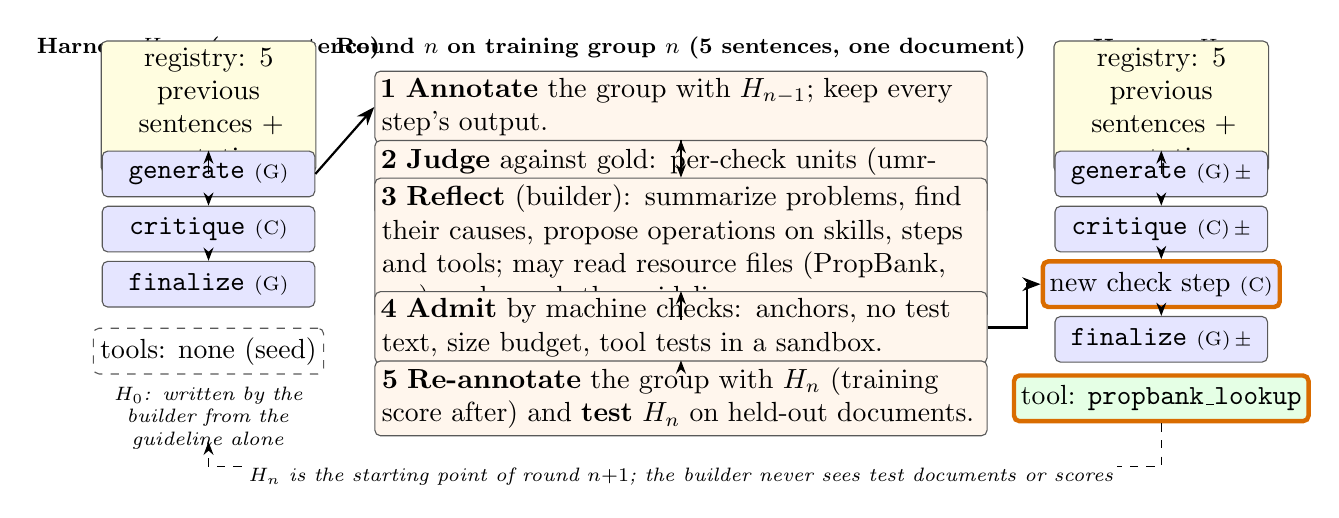
\begin{tikzpicture}[
  >=Stealth,
  box/.style={draw=black!65, rounded corners=2pt, align=center, inner sep=2.5pt, fill=white, minimum height=0.58cm},
  skill/.style={box, minimum width=2.7cm, fill=blue!10},
  rulebox/.style={box, minimum width=2.7cm, fill=black!7},
  tool/.style={box, minimum width=2.7cm, fill=green!10},
  ctx/.style={box, minimum width=2.7cm, fill=yellow!12, text width=2.55cm},
  added/.style={ultra thick, draw=orange!85!black},
  loop/.style={box, text width=7.6cm, align=left, minimum height=0.82cm, fill=orange!7},
  head/.style={font=\footnotesize\bfseries}]
% harness before
\node[head] at (0,4.55) {Harness $H_{n-1}$ (one sentence)};
\node[ctx] (r0) at (0,3.80) {registry: 5 previous sentences + annotations};
\node[skill] (g0) at (0,2.95) {\skill{generate} \scriptsize(G)};
\node[skill] (c0) at (0,2.25) {\skill{critique} \scriptsize(C)};
\node[skill] (f0) at (0,1.55) {\skill{finalize} \scriptsize(G)};
\node[box, minimum width=2.7cm, fill=white, dashed] (t0) at (0,0.70) {tools: none (seed)};
\draw[->] (r0)--(g0); \draw[->] (g0)--(c0); \draw[->] (c0)--(f0);
\node[font=\scriptsize\itshape, text width=2.8cm, align=center] at (0,-0.15) {$H_0$: written by the builder from the guideline alone};
% loop
\node[head] at (6.0,4.55) {Round $n$ on training group $n$ (5 sentences, one document)};
\node[loop] (s1) at (6.0,3.80) {\textbf{1 Annotate} the group with $H_{n-1}$; keep every step's output.};
\node[loop] (s2) at (6.0,2.90) {\textbf{2 Judge} against gold: per-check units (umrjudge / timemljudge).};
\node[loop] (s3) at (6.0,2.00) {\textbf{3 Reflect} (builder): summarize problems, find their causes, propose operations on skills, steps and tools; may read resource files (PropBank, \ldots) and search the guideline.};
\node[loop] (s4) at (6.0,1.00) {\textbf{4 Admit} by machine checks: anchors, no test text, size budget, tool tests in a sandbox.};
\node[loop] (s5) at (6.0,0.10) {\textbf{5 Re-annotate} the group with $H_n$ (training score after) and \textbf{test} $H_n$ on held-out documents.};
\foreach \a/\b in {s1/s2,s2/s3,s3/s4,s4/s5} {\draw[->] (\a)--(\b);}
% harness after
\node[head] at (12.1,4.55) {Harness $H_n$};
\node[ctx] (r1) at (12.1,3.80) {registry: 5 previous sentences + annotations};
\node[skill] (g1) at (12.1,2.95) {\skill{generate} \scriptsize(G)\,$\pm$};
\node[skill] (c1) at (12.1,2.25) {\skill{critique} \scriptsize(C)\,$\pm$};
\node[skill,added] (n1) at (12.1,1.55) {new check step \scriptsize(C)};
\node[skill] (f1) at (12.1,0.85) {\skill{finalize} \scriptsize(G)\,$\pm$};
\node[tool,added] (t1) at (12.1,0.10) {tool: \texttt{propbank\_lookup}};
\draw[->] (r1)--(g1); \draw[->] (g1)--(c1); \draw[->] (c1)--(n1); \draw[->] (n1)--(f1);
% flows
\draw[->,thick] (g0.east) -- (s1.west);
\draw[->,thick] (s4.east) -- ++(0.5,0) |- (n1.west);
\draw[->,dashed] (t1.south) -- ++(0,-0.55) -| (0,-0.55) -- (0,-0.45);
\node[font=\scriptsize\itshape, fill=white, inner sep=1.5pt] at (6.0,-0.90) {$H_n$ is the starting point of round $n{+}1$; the builder never sees test documents or scores};
\end{tikzpicture}
\caption{\sys. Left: the seed harness annotates one sentence at a time; each step sees the previous five sentences with their annotations. Middle: one round of recursive self-improvement on a group of five gold sentences. Right: the next version; skills are edited ($\pm$), and steps and tools may be added (orange), e.g.\ a PropBank lookup the builder writes after it learns that frame files exist. G and C are the generator and critic models of a configuration.}
\label{fig:overview}
\end{figure*}


\subsection{Overview}
\label{sec:overview}

\sys turns an annotation guideline and a few annotated sentences into an annotator without training any model. The method is independent of the annotation scheme: a scheme supplies its guideline, an output format with a parser, a fine-grained judge, and optionally resource files; everything else is shared (Figure~\ref{fig:overview}).

\paragraph{Annotator.} An annotator is a harness $H=(S,T,G,R)$ run by language models: \emph{skills} $S$, the instructions of each model step; \emph{tools} $T$, typed Python functions a step may call; a \emph{chain} $G$, the order of the steps and the model that runs each; and \emph{rule steps} $R$, code that rewrites an annotation without a model. Each step receives the input text, the current annotation, and unresolved findings from earlier steps. A \emph{rewrite} step produces a complete annotation, a \emph{check} step identifies problems and proposes fixes for the next rewrite step, and a rule step runs code. The final annotation is the last one that parses. Every step receives the same output format; all other instructions are learned.

\paragraph{Seed.} The builder model reads the guideline and writes the seed harness $H_0$: three steps, \skill{generate} (writes the annotation), \skill{critique} (lists problems) and \skill{finalize} (rewrites the annotation with the findings), each a checklist of at most 8{,}000 characters. The builder sees no annotated data, and the seed has no tools.

\paragraph{Recursive self-improvement.} Training data come as groups of five consecutive sentences of one document. Round $n$ turns $H_{n-1}$ into $H_n$ with group $n$ (\S\ref{sec:rsi}): annotate the group, score it with the judge, let the builder summarize the problems, reflect on their causes and propose operations on skills, steps and tools, admit the operations that pass machine checks, and annotate the group again. Each $H_n$ is tested on held-out documents, which the builder never sees.

\paragraph{Judge.} The builder needs to know which part of the scheme each error belongs to. A judge aligns the predicted annotation with the gold one and scores a set of checks, each covering one part of the scheme (for example, node concepts, argument roles, attribute values, or one type of link). It returns \emph{units}, each with a verdict (correct, wrong, missing, extra), the sentence, and the gold and predicted elements. The judges we use are described in \S\ref{sec:benchmarks}.

\subsection{The harness and its improvement}
\label{sec:rsi}

\paragraph{Representation.} A harness version is a directory of plain files: \texttt{harness.yaml} (the chain: each step's name, kind, model and tools), one Markdown skill per model step, and one Python module per tool and per rule step. A version is immutable; round $n$ copies $H_{n-1}$ and edits the copy. A configuration names two models: the generator G runs \skill{generate} and \skill{finalize}, the critic C runs \skill{critique}, and a step the builder adds names which of the two runs it.

\paragraph{Resources.} The annotating steps see only their input. Tools read resource files through one module. The builder receives a manifest of these files (for example lexicons, lists of labels and the guideline itself) and may open them while it reflects. It receives no instruction about what to build: the seed has no tools, and every tool is the builder's own design.

\paragraph{One round.} (1) \emph{Annotate}: $H_{n-1}$ annotates the five sentences of group $n$; the sentences before the group are given with their gold annotations as context. The trace keeps every step's output and findings. (2) \emph{Judge}: the judge scores the group and lists the units that are not correct. (3) \emph{Reflect}: one builder call receives the output format, the harness (chain, all skills with their sizes, all tools), the resource manifest, the changes and training scores of earlier rounds (never a test score), and, for each sentence, its gold annotation, every step's output and its incorrect units. It returns \emph{problems} (error patterns with evidence and the step to fix), a \emph{reflection} (why they happen and what to change), \emph{operations}, and \emph{suggestions} that the operations cannot express. During the call the builder can list and read resource files and search the guideline. (4) \emph{Admit}: operations are applied in order to a copy of $H_{n-1}$ when they pass the machine checks. (5) \emph{Re-annotate} the group with $H_n$, and test $H_n$ on held-out documents.

\paragraph{Operations.} \texttt{edit\_skill} modifies, inserts or deletes text at an anchor that occurs exactly once; \texttt{rewrite\_skill} replaces a skill to consolidate it; \texttt{add\_step} inserts a check, rewrite or rule step after an existing step, and \texttt{delete\_step} removes one (at most five model steps); \texttt{add\_tool}, \texttt{replace\_tool} and \texttt{delete\_tool} manage tools, and \texttt{set\_step\_tools} assigns tools to steps.

\paragraph{Admission.} Machine checks decide admission; there is no reviewer model, so a second opinion cannot block a new tool or step. No text may copy a span of a test sentence (eight characters in scripts without word spaces, six words otherwise). A skill may hold at most 10{,}000 characters; an edit that would exceed this is rejected, and the builder is asked to consolidate with \texttt{rewrite\_skill}, which keeps the harness compact as rounds accumulate. A tool or rule may import only whitelisted modules (the resource module included), may use no file, evaluation or reflection primitives, must define one public function with type annotations and a docstring, and must pass at least three tests of its own in a separate process; a tool that fails returns once to the builder with the error. A new step follows an existing one, and the first step stays a rewrite step.

\section{Experiments}
\label{sec:setup}

\subsection{Benchmarks}
\label{sec:benchmarks}

\paragraph{UMR} Uniform Meaning Representation \citep{vangysel2021designing,bonn2024building} combines sentence-level concept and argument graphs, word alignments, and document-level temporal, modal, and coreference relations. Its guideline has 365{,}742 characters. Resources include Chinese and English PropBank frames \citep{xue2009adding,palmer2005propbank}, lists of rolesets, relations and attribute values, and the guideline itself. We evaluate Chinese and English annotation using the first UMR parsing shared task \citep{stepanek2026first}.

\paragraph{TimeML} TimeML \citep{pustejovsky2003timeml} requires recognizing events and time expressions, assigning their attributes and normalized values, and linking them with fourteen temporal relation types within and across sentences. We follow the 71-page TimeML 1.2.1 guideline \citep{sauri2006timeml}, which has 115{,}146 characters and is the only resource file, and evaluate on TempEval-3 \citep{uzzaman2013semeval}. Outputs use inline entity tags followed by temporal links. Data selection and training/test splits for both benchmarks are detailed in Appendix~\ref{app:data}.

\subsection{Judges and evaluation}
\label{sec:evaluation}

\paragraph{UMR} We use AnCast++ \citep{sun2024anchor,sun2025ancastpp} to align predicted and gold nodes, comparing concepts, senses, attributes, arguments, and document-level relations (Appendix~\ref{app:judge}). We report AnCast++ sentence-graph F (\emph{F}, the main metric) and its comprehensive score including document-level relations (\emph{Comp.}), after the cleanup of \citet{chun2024pipeline}, macro-averaged over documents. We also report the shared task's official \jumach{} score \citep{stepanek2026first,zeman2026word}, computed with \texttt{compare\_umr.pl} against the official test gold. It maps nodes through token alignment and therefore also scores alignment; its gold differs from the cleaned gold used by AnCast++ (Appendix~\ref{app:data}).

\paragraph{TimeML} We built timemljudge using TempEval-3's extent and attribute measures for events and times \citep{uzzaman2013semeval} and by extending TempEval-2's categories of temporal links \citep{verhagen2010semeval} to event--time and event--event within or across sentences, event--document time, and time--time. Each category has separate checks for which pairs are linked and whether their relations are correct. For overall evaluation we use the official TempEval-3 scorer, reporting temporal-awareness TLINK F1 (\emph{TLINK}, the main metric), event and time-expression extent F1, and time-expression value F1.

\subsection{Setup}

\paragraph{Models}
The annotators are Claude Haiku~5.5 and GPT-6.1-sol. Claude Sonnet~5.5 writes the seed and is the reflector and editor in every round. Claude models run with adaptive thinking at the Messages API's default effort (Haiku medium, Sonnet high), GPT with medium reasoning effort. Each configuration was run once, with cached answers, apart from the UMR repetitions described above.

\paragraph{Baselines and learned harnesses}
We compare three annotation approaches. The baseline \emph{guideline prompt} makes one call per sentence with the whole guideline and the sentence, using Haiku, Sonnet or GPT, without earlier sentences or examples. The \emph{seed harness $H_0$} uses the three steps written from the guideline, with all four Haiku/GPT generator--critic pairs and with Sonnet in both roles. \emph{\sys} runs ten rounds of RSI with Haiku in both roles, evaluating $H_0,\ldots,H_{10}$. We then transfer $H_{10}$ unchanged to the other generator--critic pairs and to Sonnet; pairwise transfer comparisons use the same two documents per benchmark. For TimeML, the main trajectory trains on platinum documents outside the test set and a second trajectory on TBAQ-cleaned. All approaches receive the same output-format instructions.

\paragraph{Guideline access and harness ablations}
To compare ways of applying the guideline, the \emph{guideline-through-tools} variant supplies only its address and lets the model search and read it, together with UMR resource files; Haiku runs on all test documents and GPT on two per benchmark. To isolate instruction refinement, a \emph{guideline-only round} starts from the guideline prompt and permits only edits or rewrites, with no steps, tools, rules, or length limit. To isolate harness components, we run two \emph{restricted RSI} variants for two rounds each: one disables tool operations, the other rule steps. For TimeML we also test an explicit linking step (\S\ref{sec:link}).

\paragraph{Prior systems}
We re-score earlier systems on exactly our test documents from their released outputs: the two UMR shared-task systems \citep{heinecke2026orange,devergnette2026sema}, fine-tuned on the shared task's training data, of which Orange is best on both Chinese and English; and the TempEval-3 end-to-end systems \citep{uzzaman2013semeval}, of which ClearTK-2 \citep{bethard2013cleartk} is best on temporal awareness and is the best earlier system we compare with. The organizers also report TIPSem \citep{llorens2010tipsem} as a reference that scores higher, and they separate it from the participants because some annotators used it to pre-label the platinum data \citep[\S2.2, \S5]{uzzaman2013semeval}; on our documents 73\% of the gold TLINK pairs are pairs that TIPSem links (ClearTK-2: 26\%). We report TIPSem as a reference, not as the state of the art.

\section{Results}
\label{sec:results}

\begin{table*}[t]
\centering\small
\setlength{\tabcolsep}{3.6pt}
\begin{tabular}{@{}lrlcccccccc@{}}
\toprule
Doc & Sent. & Annotated by & Zero-shot & Seed $H_0$ & Learned & $\Delta$ F & Seed & Learned & $\Delta$ C & Trained \\
 & & & prompt F & F & F & & C & C & & on it, F \\
\midrule
0001 & 51 & $H_{0}$ & 31.0 & 45.1 & -- & -- & 40.5 & -- & -- & 77.5 \\
0002 & 60 & $H_{1}$ & 31.1 & 49.4 & 61.1 & +11.8 & 44.1 & 56.2 & +12.1 & 77.3 \\
0003 & 31 & $H_{2}$ & 32.3 & 45.3 & 57.2 & +11.9 & 41.3 & 55.4 & +14.1 & 84.4 \\
0004 & 59 & $H_{3}$ & 33.5 & 42.9 & 52.4 & +9.5 & 39.3 & 49.7 & +10.4 & 72.4 \\
0005 & 40 & $H_{4}$ & 32.3 & 48.0 & 58.5 & +10.5 & 44.4 & 57.1 & +12.7 & 79.7 \\
0006 & 35 & $H_{5}$ & 23.6 & 49.3 & 56.1 & +6.8 & 40.4 & 49.2 & +8.8 & 81.0 \\
0007 & 82 & $H_{6}$ & 32.6 & 46.4 & 65.5 & +19.1 & 42.3 & 59.6 & +17.3 & 85.4 \\
0008 & 10 & $H_{7}$ & \gapcell{} & 57.1 & 56.4 & $-$0.8 & 52.5 & 53.7 & +1.2 & 92.7 \\
0009 & 10 & $H_{8}$ & \gapcell{} & 59.7 & 68.0 & +8.3 & 55.2 & 65.3 & +10.1 & 99.2 \\
0010 & 12 & $H_{9}$ & \gapcell{} & 51.2 & 55.2 & +4.0 & 45.7 & 50.2 & +4.5 & 92.5 \\
0011 & 25 & $H_{10}$ & \gapcell{} & \gapcell{} & 53.4 & \gapcell{} & \gapcell{} & 48.5 & \gapcell{} & -- \\
\midrule
Mean, 9 paired documents & & & -- & 49.9 & 58.9 & +9.0 & 45.0 & 55.2 & +10.1 & \\
Mean, 0002--0007 & & & 30.9 & 46.9 & 58.5 & +11.6 & & & & \\
\bottomrule
\end{tabular}
\caption{Sequential (test-then-train) evaluation on Chinese UMR. Document $n$ is annotated by the harness built from documents $1..n{-}1$ (``Learned''), then used to improve it. ``Seed'' is $H_0$ on the same document, the paired control. ``Zero-shot prompt'' is one call per sentence with no harness (sentence graph only, so only F is comparable). F = AnCast++ sentence F; C = comprehensive score (sentence graphs plus document-level relations). The last column is the harness trained on the document itself (training fit, not generalization). Document 0001 has no earlier harness; 0011 has no seed run yet; zero-shot is missing for 0008--0011.}
\label{tab:prequential}
\end{table*}


\begin{figure*}[t]
\centering
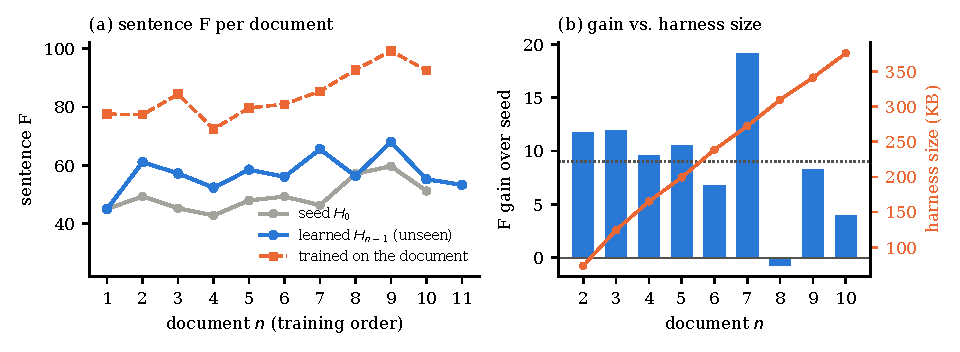
\includegraphics[width=\textwidth]{figures/curve.pdf}
\caption{(a) Sentence F per document in training order: seed harness, learned harness that has not seen the document, and the harness after three rounds on it. (b) Gain of the learned harness over the seed per unseen document (bars; dotted: mean) and the size of the harness that annotated it (line).}
\label{fig:curve}
\end{figure*}

\subsection{The learned harness is better on unseen documents}
\label{sec:main}

On the documents that also have the zero-shot prompt (0002--0007; Table~\ref{tab:prequential}), the systems form a ladder: \zeroMeanZ{} F for one call per sentence, \seedMeanZ{} for the seed harness, \firstMeanZ{} for the learned harness. Over the \nPaired{} documents with a seed control, the learned harness gains \gainF{} F (95\% CI \gainFLo--\gainFHi; Wilcoxon $p=$~\gainFWilcoxon) and improves \gainFPos{} of them; on the comprehensive score it gains \gainC{} (\gainCLo--\gainCHi) and improves all \gainCPos{} ($p=$~\gainCWilcoxon). Of \nSentPaired{} complete-case paired sentences, \sentBetter\% improve and \sentWorse\% decline by more than one Smatch point (mean +\sentGain, \sentGainLo--\sentGainHi). The one document that does not improve, 0008 (\gainMin), has ten sentences.

\paragraph{Training fit is not generalization.}
Three rounds on a document raise its own F by \trainFitGain{} points, to \afterMean{} on average and up to \afterMax, against \gainF{} on the next, unseen document (Figure~\ref{fig:curve}a). The leakage guard restricts some verbatim overlap, not learning one document's particular conventions. Evaluated on its training documents, the same loop would look three times better.

\subsection{Against baselines with the same gold}
\label{sec:baselines}

\begin{table}[t]
\centering\small
\setlength{\tabcolsep}{4pt}
\begin{tabular}{@{}lccr@{}}
\toprule
System (gold: 0001--0004) & F & C & Calls/sent. \\
\midrule
Zero-shot prompt & \gapcell & -- & 1 \\
Few-shot, $k{=}30$ & \gapcell & \gapcell & 3 \\
Guideline-only refinement & \gapcell & \gapcell & 1 \\
Procedural harness & \gapcell & \gapcell & dozens \\
\midrule
Seed harness $H_0$ & \gapcell & \gapcell & 3 \\
Learned $H_4$ (and $H_1$, $H_{10}$) & \gapcell & \gapcell & 3 \\
\bottomrule
\end{tabular}
\caption{Planned held-out set (20 documents not used to train this harness), same gold budget for all trained systems. \gap{G1--G4}}
\label{tab:heldout}
\end{table}

The held-out comparison is pending (Table~\ref{tab:heldout}). One matched comparison exists: trained on 0001--0004 with the same models, the learned harness scores \matchedCrit{} F on document 0005 and the procedural harness \matchedTree{}; the procedural seed starts higher there (\treeSeedFive{} vs.\ 48.0), so the learned gains are +\critGainFive{} and +\treeGainFive{} (one document; the procedural harness had 10 rounds, ours 12; Appendix Table~\ref{tab:matched}).

\subsection{Where the gains come from}
\label{sec:where}

\paragraph{Stage-wise generator and checker scores.}
Scoring the graph after each step (Appendix Table~\ref{tab:critique}) shows that the learned \skill{generate} alone is \genGain{} F better than the seed's on unseen documents, and \skill{critique} adds \critFirst{} on top (\critFirstMin{} to +\critFirstMax), less than the \critSeed{} it adds to the seed's draft; on the document it was trained on it adds \critAfter. Most of the observed sequential gain is already present at the generator stage. These stage-wise comparisons do not isolate the causal contribution of updating each skill, because the generator and checker were revised jointly. A variant with five specialized checks shows this more sharply: the checks add +\refineTrainMin{} to +\refineTrainMax{} on their training documents and \refineUnseen{} on unseen ones (Appendix Table~\ref{tab:refine}). At annotation time a checker has no gold, only what it was told, as self-correction studies would predict \citep{huang2024large,kamoi2024when}.

\begin{figure}[t]
\centering
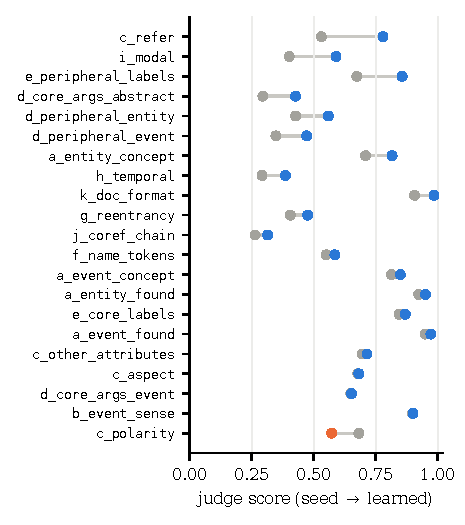
\includegraphics[width=\columnwidth]{figures/category.pdf}
\caption{Judge score per check on unseen documents: seed (grey) and learned harness (blue; orange where lower), mean over \nPaired{} documents.}
\label{fig:category}
\end{figure}

\paragraph{Gains by evaluator check.}
By judge check (Figure~\ref{fig:category}), the largest gains are on the scheme's conventions: pronoun person and number (+\catRefer{} points), the author's modal strength (+\catModal), non-core role labels (+\catPeriph), arguments of abstract rolesets such as \texttt{have-org-role-91} (+\catAbstract), non-core arguments of events (+\catPeriphEvent), entity concepts (+\catEntity). Little change is observed on several checks involving semantic judgments: PropBank sense (+\catSense), aspect (+\catAspect), core arguments of events (+\catCoreEvent). Coreference (+\catCoref) gains little and polarity falls (\catPolarity, few units). This pattern is consistent with learning scheme conventions, but these checks also involve semantic judgments. It does not establish an unchanged semantic capability or a capability ceiling; category counts and repeated, targeted comparisons are needed to test that interpretation.

\subsection{Tools are proposed rarely and admitted never}
\label{sec:tools}

In \nRounds{} rounds the builder proposed \nProposals{} tools and no steps; the reviewer rejected all three. \texttt{check\_umr\_graph} checked attribute values, entity types and role names; the reviewer kept the purely mechanical checks (colon-prefixed or misspelled closed-list values, parse failures, duplicate variables) and judged the rest to be missing conventions that belong in the instructions. \texttt{check\_umr\_form} flagged bare constants and aspect on discourse rolesets; the second part contradicted the builder's own earlier rule. \texttt{check\_doc\_relations} checked coreference on name nodes and double temporal parents, but one test contradicted a convention of \skill{document}. Each time a sound core was lost, because rejected proposals are not revised. Without the reviewer (the TimeML and manifesto runs), the builder changes tools or rules in most rounds \gap{G7: does admitting them help?}.

\subsection{Instruction growth without a clear increase in sequential gains}
\label{sec:growth}

This trajectory shows no clear increase in gain with the number of preceding documents (Figure~\ref{fig:curve}b): +\gainFirstHalf{} on average for documents 2--6, +\gainSecondHalf{} for 7--10 (Spearman $\rho=$~\gainRho, $p=$~\gainRhoP). The harness grows from \sizeSeed{} to \sizeLast{}\,KB (\sizeGen{} in \skill{generate}, \sizeCrit{} in \skill{critique}, \sizeDoc{} in \skill{document}), \sizePerRound{}\,KB per round. Of \nEditsApplied{} applied edits, \nModify{} modify, \nAdd{} add and \nDelete{} delete (Appendix Table~\ref{tab:edits}): nothing rewards a shorter harness. The correlation does not establish a flat learning curve, since document difficulty and order change along with the harness. Whether this pattern reflects what one document can teach, from interference among accumulated rules, or from length is open; held-out scores of $H_1$ to $H_{10}$ and a consolidation pass under a size budget would separate these \gap{G5, G6}.

\begin{table}[t]
\centering\small
\setlength{\tabcolsep}{2pt}
\begin{tabular}{@{}llrrrr@{}}
\toprule
Builder / annotator & Harness & $n$ & Seed & Learned & $\Delta$ \\
\midrule
Opus / Sonnet 5.5 & ours$^s$ & 9 & 49.9 & 58.9 & +9.0 \\
Opus / Sonnet 5.5 & proc. & 2 & 45.5 & 52.9 & +7.4 \\
DeepSeek (no thinking) & proc. & 5 & 32.5 & 37.6 & +5.2 \\
Qwen3.5-9B & proc.$^s$ & 13 & 17.6 & 16.3 & $-$1.4 \\
\midrule
Qwen3.5-27B & proc.$^s$ & \gapcell{} & \gapcell{} & \gapcell{} & \gapcell{} \\
Opus / small model & ours & \gapcell{} & \gapcell{} & \gapcell{} & \gapcell{} \\
Small model / Sonnet & ours$^s$ & \gapcell{} & \gapcell{} & \gapcell{} & \gapcell{} \\
\bottomrule
\end{tabular}
\caption{Seed vs.\ learned harness on unseen documents, sentence F. One name: the same model builds and annotates. proc.: procedural harness. $^s$sequential protocol; otherwise a few training documents and separate test documents. DeepSeek's seed reaches 49.1 F with thinking on vs.\ 35.9 off (document 0002).}
\label{tab:models}
\end{table}


\subsection{A weaker joint builder--annotator configuration}
\label{sec:models}

The gain holds for the procedural harness with the same models and for DeepSeek building and annotating without thinking (Table~\ref{tab:models}). With Qwen3.5-9B building and annotating over \qwenSmallN{} documents, the learned harness is worse than the seed (\qwenSmallGain{} F on average; better on \qwenSmallPos{} documents), and the decline deepens (+\qwenSmallFirst{} in the first half, \qwenSmallSecond{} in the second); two independent seed runs differ by \qwenSeedNoise{} F per document, which limits interpretation of individual changes. The available reruns do not establish the significance of the trajectory. On agentic tasks, by contrast, a 9B model's harness updates were as useful as a frontier model's \citep{lin2026harness}. Whether builder or annotator matters more here is not yet separated \gap{G8}.

\subsection{Ablations of the loop}
\label{sec:ablation}

\begin{table}[t]
\centering\small
\setlength{\tabcolsep}{3pt}
\begin{tabular}{@{}lccc@{}}
\toprule
Variant & $\Delta$F seq. & $\Delta$F held-out & KB \\
\midrule
\sys & \gapcell & \gapcell & \gapcell \\
\quad no attribution (one list) & \gapcell & \gapcell & \gapcell \\
\quad whole-skill rewrites & \gapcell & \gapcell & \gapcell \\
\quad \skill{generate} only & \gapcell & \gapcell & \gapcell \\
\quad no reviewer & \gapcell & \gapcell & \gapcell \\
\quad + test edits on held-in docs & \gapcell & \gapcell & \gapcell \\
\quad + consolidation & \gapcell & \gapcell & \gapcell \\
\quad other document orders & \gapcell & \gapcell & \gapcell \\
\bottomrule
\end{tabular}
\caption{Planned matched-budget ablations: sequential gain on 0002--0005 and gain on the held-out set. All rows must be recomputed on this common protocol; the reported full-run gain over 0002--0010 is not a baseline for this subset. \gap{G9}}
\label{tab:ablation}
\end{table}

Table~\ref{tab:ablation} lists the ablations that test the design: whether attribution to a skill matters (one undivided problem list), whether typed edits matter (each round rewrites a skill in full, as guideline refinement does), whether the checking step is needed, whether the reviewer helps or only blocks, whether testing each edit before keeping it \citep{zhang2026self,kim2026refining} closes the training-fit gap, whether consolidation lifts the plateau, and how much document order matters \gap{G9: to run}.

\subsection{Beyond UMR}
\label{sec:beyond}

The same loop builds a TimeML annotator for TempEval-3 \citep{uzzaman2013semeval} and a coder that assigns manifesto sentences one of the eight policy domains of the Manifesto Project scheme \citep{lehmann2026manifesto}, with variant protocols that omit the model reviewer and permit rule and registry changes (Appendix~\ref{app:other}; finished baselines in Tables~\ref{tab:timeml} and~\ref{tab:manifesto}). On both test sets the seed harness is below the zero-shot prompt (TimeML event F1 74.5 vs.\ 80.7; manifesto accuracy 63.8 vs.\ 65.0), so the learned harness must first make up for its own seed. \gap{G10, G11: learned harness on both test sets; sequential gains.}

\section{Analysis}
\label{sec:analysis}

\paragraph{What the builder writes.}
In its first round the builder found 752 divergences in document 0001, read 250 of them (the cap), and sorted them into six patterns: form (colon-prefixed or capitalized values, abbreviated modal strengths, AMR role names such as \texttt{:time} for UMR's \texttt{:temporal}); named-entity types and tokens; discourse relations written as reified rolesets (\texttt{have-reason-91}) rather than edges; reported speech; Chinese granularity (which compounds split, which adverbs, demonstratives and classifiers keep a node); and document-level defaults for dates and temporal relations. These are the topics a human guideline spends its pages on, and they match the checks that improve on unseen documents (Appendix~\ref{app:edits} shows edits verbatim).

\paragraph{What the builder asks for and cannot do.}
Each round may also list changes outside the instructions, which the loop does not apply. We coded all \nSuggestions{} (Appendix~\ref{app:suggestions}). \sugGold{} concern the gold: conventions that differ between documents or annotators (the argument order of the concession roleset, whether title marks belong to a name, how names are split into tokens, which person type is used), usually with a decision not to learn from them yet, and outright errors such as undefined variables or an unbalanced bracket. \sugRule{} ask for deterministic code, such as normalizing attribute values or validating document-level relations against the graphs; one is the bracket fix we made by hand. \sugContext{} ask for more input to a skill (a running list of coreference chains, the genre) and \sugEval{} for evaluator changes. A builder with gold is thus also an auditor of gold, the moderation step of a human project; and by its own diagnosis much of what remains needs code and context, which the admission gate of \S\ref{sec:tools} blocked every time.

\paragraph{How the harness goes wrong.}
Beyond the training-fit gap and unbounded growth, three failure modes recur. \emph{Contradictions}: in round 2 the builder proposed a check forbidding aspect on discourse rolesets while its own round-1 rule and example required it; the reviewer caught this because it came as a tool, but edits to prose pass no such check. \emph{Following the latest document}: after 0001 the instructions said a negated event is full-negative \emph{without} \texttt{:polarity -}; the first round on 0002, whose gold marks polarity, made it require both. By $R_{111}$, disagreements between documents have become rules conditioned on genre (``in a biography only'', ``in a plot summary''). \emph{Local regressions}: since no edit is tested before it is kept, a regression surfaces only on the next document. Testing edits on held-in documents \citep{zhang2026self,wang2026do} and sending gold conflicts to people would address the last two \gap{G9}.

\paragraph{Cost.}
The seed harness costs about \$0.08 per sentence at API list prices (three calls, cached prefixes). The learned harness reads up to \sizeLast{}\,KB of instructions per sentence, mostly cached; building costs one call per sentence with an error and one planning call per round. \gap{G12: cost and latency of $H_1$, $H_4$, $H_{10}$; cost of building; time to write the seed.}

\section{Conclusion}
\label{sec:conclusion}

Complex annotation can be bootstrapped from a guideline and a few examples: without fine-tuning, an LLM that is given the guideline as a chain of steps, tools over the project's resources, and a loop that revises them against a handful of gold sentences, annotates UMR better than the fine-tuned systems of its shared task on the same documents. A long guideline alone is not enough, and neither is a one-time compression of it: the gains come from the harness, its decomposition into steps and its tools, and from recursive self-improvement with a fine-grained judge, which plays the role that moderation plays in a human annotation project. In that loop the builder model learned to edit the guideline, to write the tools the guideline presupposes, and to turn recurring decisions into code.

The same loop shows its limits. What it learns are the conventions of the gold it sees: it learned which TimeML events to link, and, from a sparser corpus, to link less; senses and arguments improved where a tool supplied the frames, but judgments that no resource supports, aspect, coreference and temporal relations, moved little; and its own suggestions are dominated by inconsistencies of the gold. This points to a different division of labor in annotation projects. A guideline can be an executable object that is tested and revised against data from the first annotated sentences on; the model maintains the instructions, tools and checks, and people decide the conventions and adjudicate the inconsistencies it surfaces. Bootstrapping a new scheme or language then starts from a working annotator rather than from an empty corpus.

\section*{Limitations}
\label{sec:limitations}

\paragraph{Scale and variance} Each test set has at most 100 sentences in four to seven documents, and every configuration was run once, in one order of training groups, with cached answers. The bootstrap intervals describe variation over test documents, not over runs of the builder or of the annotators; repeated trajectories and other group orders are needed to estimate that variance.

\paragraph{Models} The builder (Sonnet) and the main annotator (Haiku) are from one model family. Several GPT-6.1-sol conditions cover part of the test documents (the guideline prompt on UMR and most transfer pairs); Table~\ref{tab:main} marks them. Claude models ran through the Claude Agent SDK on a subscription and GPT through OpenRouter; providers' defaults and versions may change. The controls of \S\ref{sec:controls} and the TimeML link step were run for one or two rounds only.

\paragraph{Cost} An annotation with $H_{10}$ takes about three model calls per sentence (more with tool calls). With GPT-6.1-sol in both roles it cost about \$0.07 per sentence at OpenRouter's prices, so the Chinese and English part of the shared task's test set (431 sentences, of which our test sets are 194) would cost about \$31 with GPT; with Haiku on a subscription it costs no money but about \$0.22--0.30 per sentence at API-equivalent prices. Sentences of a document are annotated in order (each sees the five before it), so the longest document (100 sentences) bounds the wall-clock time at about two to three hours; the ten rounds of one trajectory, with a test after each, took about three hours.

\paragraph{Data} The English training groups come from only three fully annotated documents; most of the released English UMR data are partial conversions without aspect or document-level relations. The Chinese gold we score against differs from the shared task's own gold (Appendix~\ref{app:data}), so we report both. The TimeML results depend strongly on which gold the builder sees (\S\ref{sec:how}). Test documents may occur in the models' pretraining data.

\paragraph{Admission} Operations are admitted by machine checks only; nothing tests an edit before it is kept, so a round can make the harness worse on unseen data (Figure~\ref{fig:curves}). A held-in check of each edit, and people adjudicating the gold inconsistencies the builder reports, are natural additions.

\paragraph{Human influence} The seed builder's prompt, the reflection prompt, the operation set, the judges and the admission rules were designed by the authors. During the runs we changed the admission code twice (rule steps get one repair attempt; helper functions are allowed in tools) and restarted the trajectories from scratch each time, and we replaced the English and TimeML training pools once after finding training documents without document-level annotation.

\section*{Ethics Statement}
Automating annotation can reduce the paid work available to annotators. We see \sys as a way to start an annotation project from a working draft annotator, with people deciding conventions and adjudicating the inconsistencies the builder surfaces. UMR data are used under their CC licenses; TimeBank and AQUAINT text (LDC) is not redistributed. Model calls went to commercial APIs. Generative AI was used to run the experiments and to draft and edit this paper.


\bibliography{references}

\appendix
\section{The Judges}
\label{app:judge}
TBD
\section{Data}
\label{app:data}
TBD


\end{document}
